\section{The Mechanical System}

\subsection{The Original Components}
Most of the mechanical components on board the vehicle were installed by the SCOPE team that first worked on the vehicle in 2009 - 2010. As such, this section begins by including the original pages from the 2009 - 2010 SCOPE team report describing the mechanical system. \\ \\
%
Today, this mechanical system remains largely the same except for the following changes:

\begin{enumerate}
\item The monitor mentioned in the original SCOPE team report is the Nortec SUN-1710-P daylight-visible monitor. The current monitor on the vehicle is a standard Acer monitor
\end{enumerate}

\newpage

\includepdf[scale=0.9, pages=2, clip, trim=0mm 20mm 0mm 65mm, pagecommand={\subsection{Gas and Brake Actuation System}}]{MechSystem.pdf}
\includepdf[scale=0.9, pages=3-9, clip, trim=0mm 20mm 0mm 35mm, pagecommand={}]{MechSystem.pdf}
\includepdf[scale=0.9, pages=10, clip, trim=0mm 75mm 0mm 35mm, pagecommand={}]{MechSystem.pdf}
\includepdf[scale=0.9, pages=12, clip, trim=0mm 20mm 0mm 35mm, pagecommand={}]{MechSystem.pdf}
\includepdf[scale=0.9, pages=13, clip, trim=0mm 130mm 0mm 35mm, pagecommand={}]{MechSystem.pdf}

\newpage

\subsection{Steering System}
The steering actuation uses a pre-existing power steering assist kit that is modified to meet project requirements. This steering plan is similar to a system prototyped on the summer 2009 research vehicle, the Yamaha Rhino, and is designed by the same manufacturer. The kit required two main modifications: the addition of a more robust controllable motor and the creation of some sort of feedback method from the device. The stock motor from the power steering kit does not provide feedback and lacks sufficient power to control the vehicle in worst case conditions. Both of these issues are addressed by installing a larger motor with a built-in encoder. This solution requires several additional changes to the pre-existing kit: 

\begin{enumerate}
\item Its position in the gator
\item The motor attachment to the rest of the power steering unit
\item The motor interface with the power steering unit to deliver power.
\end{enumerate}

\noindent The motor has to deliver 150 in-lbs at the steering wheel (twice that for a sizable safety margin). The motor is limited also to 5A at 12V to remain compliant with the cRIO 9505 motor controller. The 150 in-lbs requirement was determined through experimental measurement, by turning the steering wheel from left lock to right lock and back while resting on the grass at a standstill. The motor chosen to meet these specifications is provided by Potomac Electric, and has a 4? diameter and a length of 8? with a 5/8? diameter shaft. In order to rotate the power steering kit into a more favorable position, an adapter plate was designed to fit between the power steering assembly and the brace that attaches it to the chassis. Keeping the motor in the original orientation would have required major modifications to the chassis and dashboard in order to fit the motor. Inclusion of the larger motor required development of a method for attaching it to the rest of the unit. The original motor attached to the power steering housing through an aluminum heat shrunk collar with through holes for two bolts. The diameter of the new motor made a direct analog unfeasible, requiring design a larger collar which offset the motor enough to allow use of the two existing bolt holes from the previous motor mount. Figure 20 shows this adapter.

The original motor delivered power to the steering kit through a non standard spider coupling, requiring design of a corresponding piece that fits on the new motor. The motor shaft is attached to the new spider coupling with a keyless bushing (Figure 21 shows the new coupling). When power is cut to the motor the operator has full control of the vehicle and is able
to back-drive the motor. In addition to the various adaptor pieces the motor is secured by a harness on the back of the motor. The harness is shown in Figure 22 and consists of a 4? rubber-coated u-bolt, two machined plates, a threaded rod, and a split clamp hangar which attaches to pole running through the dashboard.

\includepdf[scale=0.8, pages=16, clip, trim=0mm 20mm 0mm 80mm, pagecommand={\subsection{Steering Limit Switches}}]{MechSystem.pdf}

\includepdf[scale=0.9, pages=17, clip, trim=0mm 20mm 0mm 35mm, pagecommand={}]{MechSystem.pdf}

\noindent calibration routine to run regardless of the initial position of the steering column, as a turn in a certain direction will always hit the same sensor. Additionally, this allows the limit sensors to double as a shutoff triggers if a problem develops with the steering control software during a run, while at the same time preserving the maximum useable range of steering.

\subsection{Wheel Encoder Mount System}
To provide velocity feedback for vehicle control, the Gator utilizes an optical wheel encoder. The wheel encoder mounting consists of an ANSI 35 sprocket and chain system pictured in Figure 23. One sprocket is attached to the optical encoder shaft, and the other is driven by the driveshaft located under the utility bed on the right side of the Gator. The driveshaft sprocket was manually split and fitted with socket head cap-screws in order to mount it around the shaft without requiring major disassembly of the Gator platform. The encoder itself is bolted to a length of steel L-channel, which is in turn bolted to the frame of the gator using a pair of tap rivets. Using a sprocket chain allows the system to accommodate the slight yet inevitable misalignment that results from this assembly. Because of the tendency of sprocket chain to stretch over time, all sprocket chain systems require some way to dynamically tension the chain. In this system, tensioning is accomplished through the use of a flexible polymer sprocket ring designed to provide tension to roller chain systems without extra mounting hardware. Because of its natural elasticity, the polymer sprocket ring exerts a radial force on the sprocket chain loop, keeping the chain in tension
as it spins. Since velocity feedback will be derived from the rotary motion of the encoder, it is important to understand the ratio between encoder ticks and vehicle speed. Since the chosen encoder has 500 ticks per revolution and the sprocket system results in 16:9 gear ratio between the vehicle drive shaft and the encoder shaft, the encoder will register approximately 890 ticks per revolution of the drive shaft. There is a one-to-one correspondence between rotations of this shaft and rotations of the tires, which are approximately 23 inches in diameter. Using this a baseline and calibrating further using field testing, it was possible to establish a ratio of 3000 encoder ticks per foot of forward vehicle movement.

\includepdf[scale=1.2, pages=13, clip, trim=0mm 20mm 0mm 145mm, pagecommand={}]{MechSystem.pdf}

\includepdf[scale=0.8, pages=15, clip, trim=0mm 100mm 0mm 75mm, pagecommand={\subsection{Generator Mount} The system's gasoline generator is mounted to the rear of the Gator's utility bed by two standard ratcheting tie-down straps. The straps attach to four 800-pound working load tie- down rings which have been installed in the base of the utility bed.}]{MechSystem.pdf}

\subsection{Additional Mechanical Components}